\input{src/header}											% bindet Header ein (WICHTIG)
\usepackage{graphicx}
\usepackage{fancyvrb}

\newcommand{\dozent}{Prof. Dr. Agn`es Voisard, Nicolas Lehmann}					% <-- Names des Dozenten eintragen
\newcommand{\tutor}{Nicolas Lehmann}						% <-- Name eurer Tutoriun eintragen
\newcommand{\tutoriumNo}{10}				% <-- Nummer im KVV nachschauen
\newcommand{\projectNo}{6}									% <-- Nummer des Übungszettels
\newcommand{\veranstaltung}{Datenbanksysteme}	% <-- Name der Lehrveranstaltung eintragen
\newcommand{\semester}{SoSe 2017}						% <-- z.B. SoSe 17, WiSe 17/18
\newcommand{\studenten}{Boyan Hristov, Julian Habib}			% <-- Hier eure Namen eintragen
% /////////////////////// BEGIN DOKUMENT /////////////////////////

\begin{document}

% /////////////////////// BEGIN TITLEPAGE /////////////////////////
\begin{titlepage}
	\subject{\dozent}
	\title{\veranstaltung, \semester}
	\subtitle{\Large Übungsblatt \projectNo\\ \large\vspace{1ex} }
	\author{\studenten}
	\date{\normalsize \today}
\end{titlepage}

\maketitle								% Erstellt das Titelblatt
\vspace*{-9cm}							% rückt Logo an den oberen Seitenrand
\makebox[\dimexpr\textwidth+1cm][r]{	%rechtsbündig und geht rechts 1cm über Layout hinaus
	\includegraphics[width=0.4\textwidth]{src/fu_logo} % fügt FU-Logo ein
}
% /////////////////////// END TITLEPAGE /////////////////////////

\vspace{7cm}							% Abstand
\rule{\linewidth}{0.8pt}				% horizontale Linie										% erstellt die Titelseite

Link zum Git Repository: \url{https://github.com/BoyanH/Freie-Universitaet-Berlin/tree/master/Datenbanksysteme/Solutions/homework\projectNo}

% /////////////////////// Aufgabe 1 /////////////////////////

\section*{1. Aufgabe}

\begin{enumerate}

\item[a)]
z.z.: $R_1$ ist in 1NF $\Leftrightarrow$ alle Attribute sind atomar. \\ \\
$R_1(A,B,C,D) \subseteq A \times B \times C \times D \Rightarrow $ A,B,C,D sind atomar.

Alle Attributen in $R_1$ haben atomäre Domäne, sind also keine Relationen. Z.B. alle Einträge haben für den Attribut A die Werte $a_1, a_2, a_3$ und keine Werte wie z.B. $(a_1, a_2)$.

$\hfill \Box$

\item[b)]
z.z.: $R_1$ ist nicht in 2NF \\ \\
$R_1$ ist in 2NF $\Leftrightarrow$  $R_1$ ist in 1NF und $\forall (X \rightarrow A) \in F_{+} | A \not\in X: X \not\subset $ Superschlüssel $\lor A \subseteq$ Schlüssel.

Beweis durch Gegenbeispiel:

\begin{align*}
    FD(R_1) = \{ & \\
    & A \rightarrow B \\
    & A \rightarrow C \\
    & D \rightarrow C \\
    & BD \rightarrow A \\
    \} & \\
    \Rightarrow & \text{ AD und BD sind Superschlüssel und auch beide Kandidatschlüsseln.} \\
    & \text{Primäre Attributen sind A, B und D. }
\end{align*}

Da C kein Primärattribut ist, von A abhängig ist und da A eine Untermenge eines Schlüssels ist (AD), ist $R_1$ nicht in 2NF.

$\hfill \Box$

\item[c)]
z.z.: $R_2$  ist in 3NF $\Leftrightarrow \forall FD(X \rightarrow A):$ X ist Superschlüssel von R oder A ist Primärattribut von R

Direkter Beweis: 

\begin{align*}
    FD(R_2) = \{ & \\
    & E \rightarrow F \\
    & E \rightarrow G \\
    & FG \rightarrow E \\
    \} & \\
    \Rightarrow & \text{ E und FG sind Superschlüssel, Primärattributen sind E, F und G. }
\end{align*}

In den ersten zwei funktionalen Abhängigkeiten ist die linke Seite ein Superschlüssel, in der 3. Abhängigkeit ist die rechte Seite ein Primärattribut.
$\Rightarrow R_2$ ist in 3NF.

$\hfill \Box$

\item[d)]

z.z: $R_2$ ist in BCNF $\Leftrightarrow \forall X \rightarrow A \in F_{+}:$ X ist Superschlüssel.

Direkter Beweis: 

\begin{align*}
    FD^{+}(R_2) = \{ & \\
    & E \rightarrow F \\
    & E \rightarrow G \\
    & E \rightarrow FG \\
    & FG \rightarrow E \\
    \} &
\end{align*}

Da wir schon aus c) kennen, dass E und FG Superschlüssel sind und da diese alle mögliche linke Seiten von einer funktionalen Abhängigkeit sind, ist $R_2$ in Boyce-Codd Normalform (BCNF).

$\hfill \Box$

\end{enumerate}

\section*{2. Aufgabe}

\begin{enumerate}

\item[a)]
Mit dem Algorithmus aus der Vorlesung für "Well-behaved 3NF Decomposition"

\begin{align*}
    FD(R_3) = \{ & \\
    & H \rightarrow JK \\
    & I \rightarrow HJ \\
    & K \rightarrow L \\
    \} &
\end{align*}

\begin{enumerate}
\item[1.] For each FD (X $\rightarrow$ A) in F 
create a relation with schema (XA). \\

\begin{align*}
    (HJK), (IHJ), (KL)
\end{align*}

\item[2.] If none of the keys appears in one of the schemas of 1
then add a relation with schema Y, with Y a key. \\

$\Rightarrow$ fertig, da H ein Schlüssel ist und in (HJK) vorhanden ist.

\item[3.] If for relations created in 1. there exists a relation R1 whose
schema is included in the schema of another relation, then remove
R1. \\

Alles ist in Ordnung, die Attributen von keinem Schema sind eine Untermenge von den Attributen eines anderen Schemas.

\item[4.] Replace relations (X A1), ..., (X Ak)
with a single relation (X A1 ... Ak).

\begin{align*}
     & (HJK) \land (IHJ) \Rightarrow (HJIK)
\end{align*}

\end{enumerate}



Gute Zerlegung: $R_{31}(H,J,I,K)$ und $R_{32}(K,L)$

\item[b)]

\begin{align*}
    & R_{31} \cap R_{32} \equiv K \\
    & R_{31} - R_{32} \equiv HJI
    & R_{32} - R_{31} \equiv L \\ \\
    & R_{31} \cap R_{32} \rightarrow KL  \text{ (wegen K $\rightarrow$ L) }
        \rightarrow L \equiv R_{31} - R_{32} \\
    \Rightarrow & \text{ Unsere Zerlegung ist verlustlos} 
\end{align*}

\item[c)]

\begin{align*}
    & FD(R_{31}) = \{ H \rightarrow JK, I \rightarrow HJ \} \\
    & FD(R_{32}) = \{ K \rightarrow L \} \\
    & FD(R_{31}) \cup FD(R_{32}) \equiv \{ H \rightarrow JK, I \rightarrow HJ, K \rightarrow L \} \equiv FD(R_3) \\
    \Rightarrow & \text{ Unsere Zerlegung ist abhängigkeitserhaltend}
\end{align*}

\item[d)]
Da wir dieses Algorithmus benutzt haben, ist jede davon entstandene Relation in 3NF. Wegen b), c) und d) ist die Zerlegung gut. Für $R_{32}$ sind H und I Schlüssel und an alle funktionalen Abhängigkeiten auf der linken Seite vorhanden, deswegen ist $R_{32}$ in 3NF. $R_{32}$ hat nur eine funktionale Abhängigket und nur 2 Attributen, ist deswegen trivialerweise in 3NF.


\end{enumerate}

\section*{3. Aufgabe}

\begin{enumerate}

    \item[a)]
    Aus jedem Item kann man durch eine Hash-Funktion ein Hash erzeugen durch mathematische Umformungen aus allen Suchschlüssel. Mehrere Items werden in dem selben Bucket gespeichert (nacheinandere folgende Blöcke im Speicher) wenn die Hashfunktion das gleiche Hash aus ihren Suchschlüssel erzeugt. Danach, beim Suchen von Lösch / Einfüge / Lese Position müssen alle Einträge in dem entsprechenden Bucket nach einander geprüft werden. Deswegen erzeugen gute Hashfunktione randomisierte Hashes, damit es ungefähr genau so viele Items pro Bucket gibt.

    \item[b)]
    In einem Dense-Index gibt es Indizes für alle Suchschlüsselwerte. Z.b. wenn das Attribut A ein Primärindex ist, gibt es für alle mögliche Werte von A ein Index, die Einträge mit dem gleichen Wert von A stehen nach einander im Speicher.

    Der Sparse-Index hat nur für gewählte Werte von den Suchschlüssel Indizes. Dabei müssen aber immer die Einträge im Speicher nach dem Primärindex sortiert werden. Damit sucht man nach dem Index des alphabetisch größten kleineren Wert und muss dann alle weitere Einträge durchsuchen, um den Item zu finden. Dabei haben wir viel speicher für den Index gespart, die Suchzeiten haben sich aber vergrößert. Ein gutes Balance zwischen den beiden ist zu finden.

    \item[c)]
    Ein Multilevel-Index ist ein Index, wo das unterste Niveau ein Dense-Index ist und darüber noch n Stufen von Sparse-Index existieren. So kann man viel Schneller suchen ($log_2(n)$, da es so viele Schritten vom Wurzel zu den Blätter in einem balancierten Baum mit n Blätter gibt). Die Blätter eines $B^{+}$ Baums sind die äußeren Indizes und die restliche Knoten die innere Indizes. Diese Struktur darf man aber nur dann verwenden, wenn die Suchschlüssel sortierbar sind, da man sonst kein $B^{+}$ oder überhaupt kein Suchbaum konstruieren kann.

    \item[d)]
    "Fixed Length Records" \\
    Sei 3 die Länge eines Records \\ \\
    \begin{tabular}{ l | l | l | l |}
    \hline
    \#record & Film Name & Actor's Name & Actor's Address \\ \hline
    0 & Fremde Gewässer & Thomas Depp & Paris \\ \hline
    1 & Fremde Gewässer & Linda Cruz & Los Angeles \\ \hline
    2 & Furious Sixteen & Martin Diesel & Detroid \\ \hline
    3 & Furious Sixteen & Grünther Walker & New York
    \end{tabular}

    "Variable Length Records" \\ \\
    \begin{tabular}{| l | l | l | l | l | l | l |}
    \hline
    \#record & Film Name & Actor's Name & Actor's Address & Actors's Name & ... & ... \\ \hline
    0 & Fremde Gewässer & Thomas Depp & Paris & Linda Cruz & Los Angeles & $\perp$ \\ \hline
    1 & Furious Sixteen & Martin Diesel & Detroid & Grünther Walker & New York & $\perp$ \\ \hline
    \end{tabular}

    Mit Hilfe von Pointer \\

    \includegraphics[width=\textwidth]{pointerRepresentation.png}

\end{enumerate}

\section*{Aufgabe 3.}

\begin{enumerate}

\item[a)]

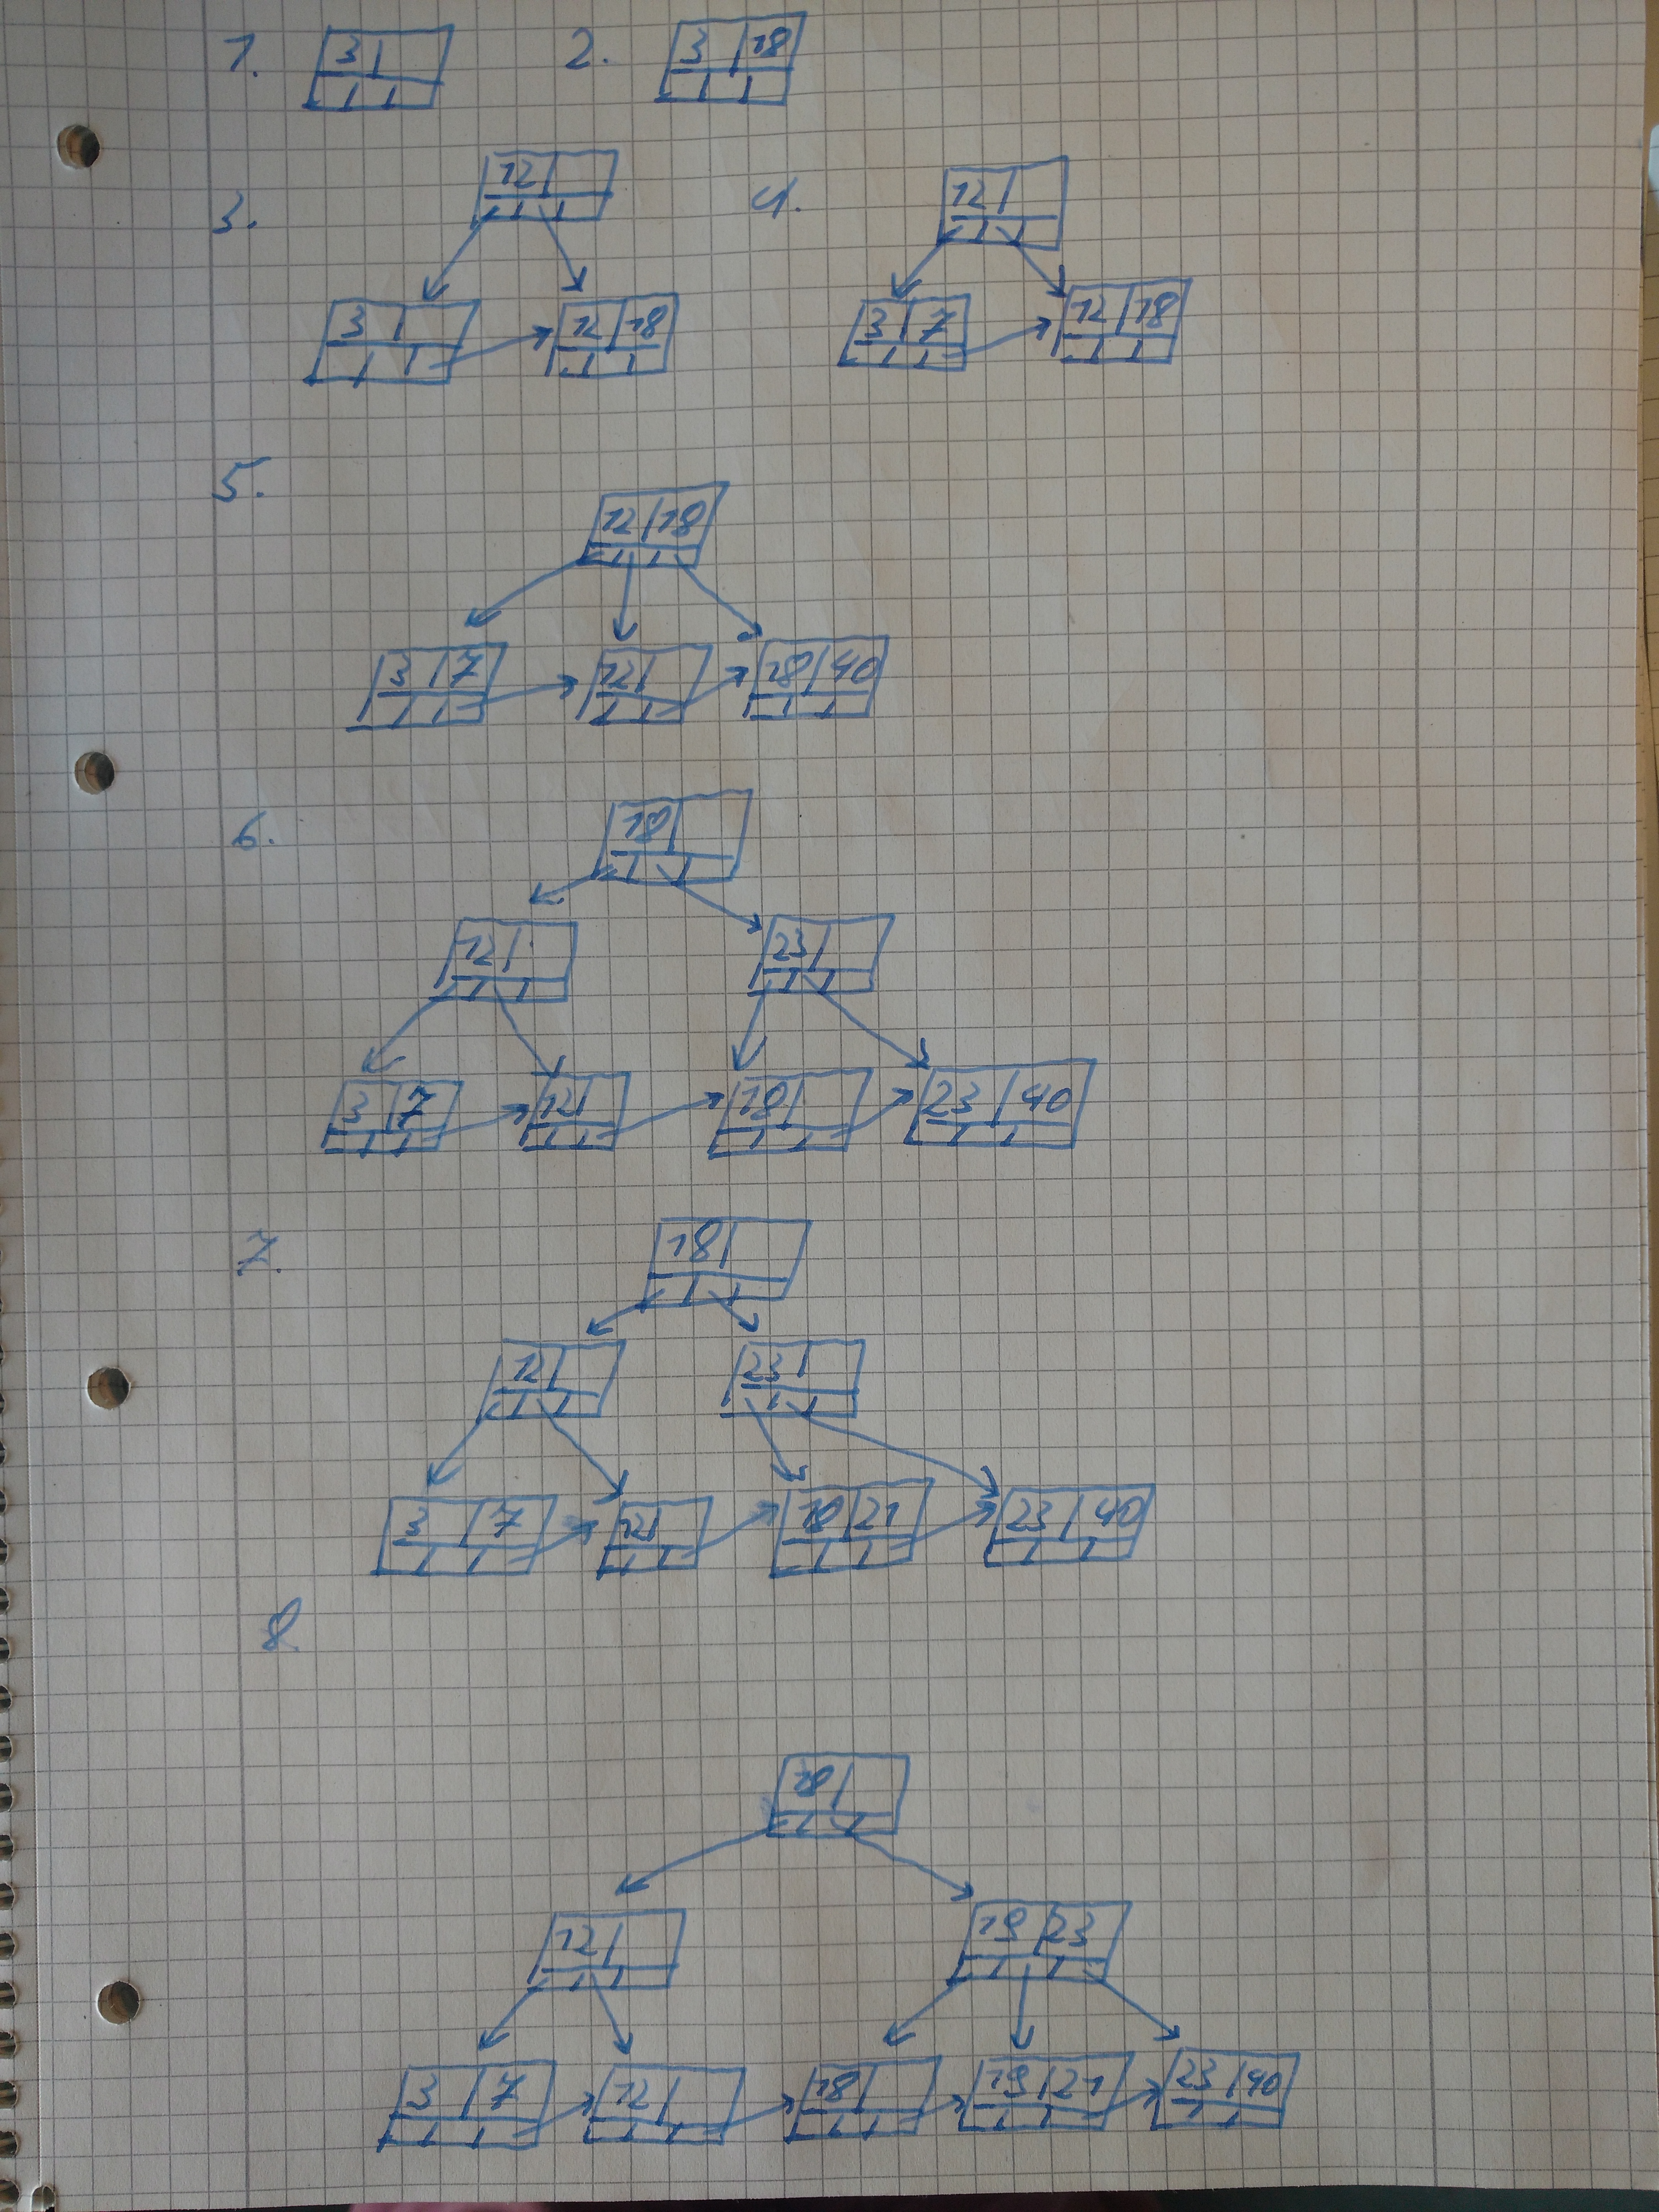
\includegraphics[width=\textwidth]{./images/a1.jpg}
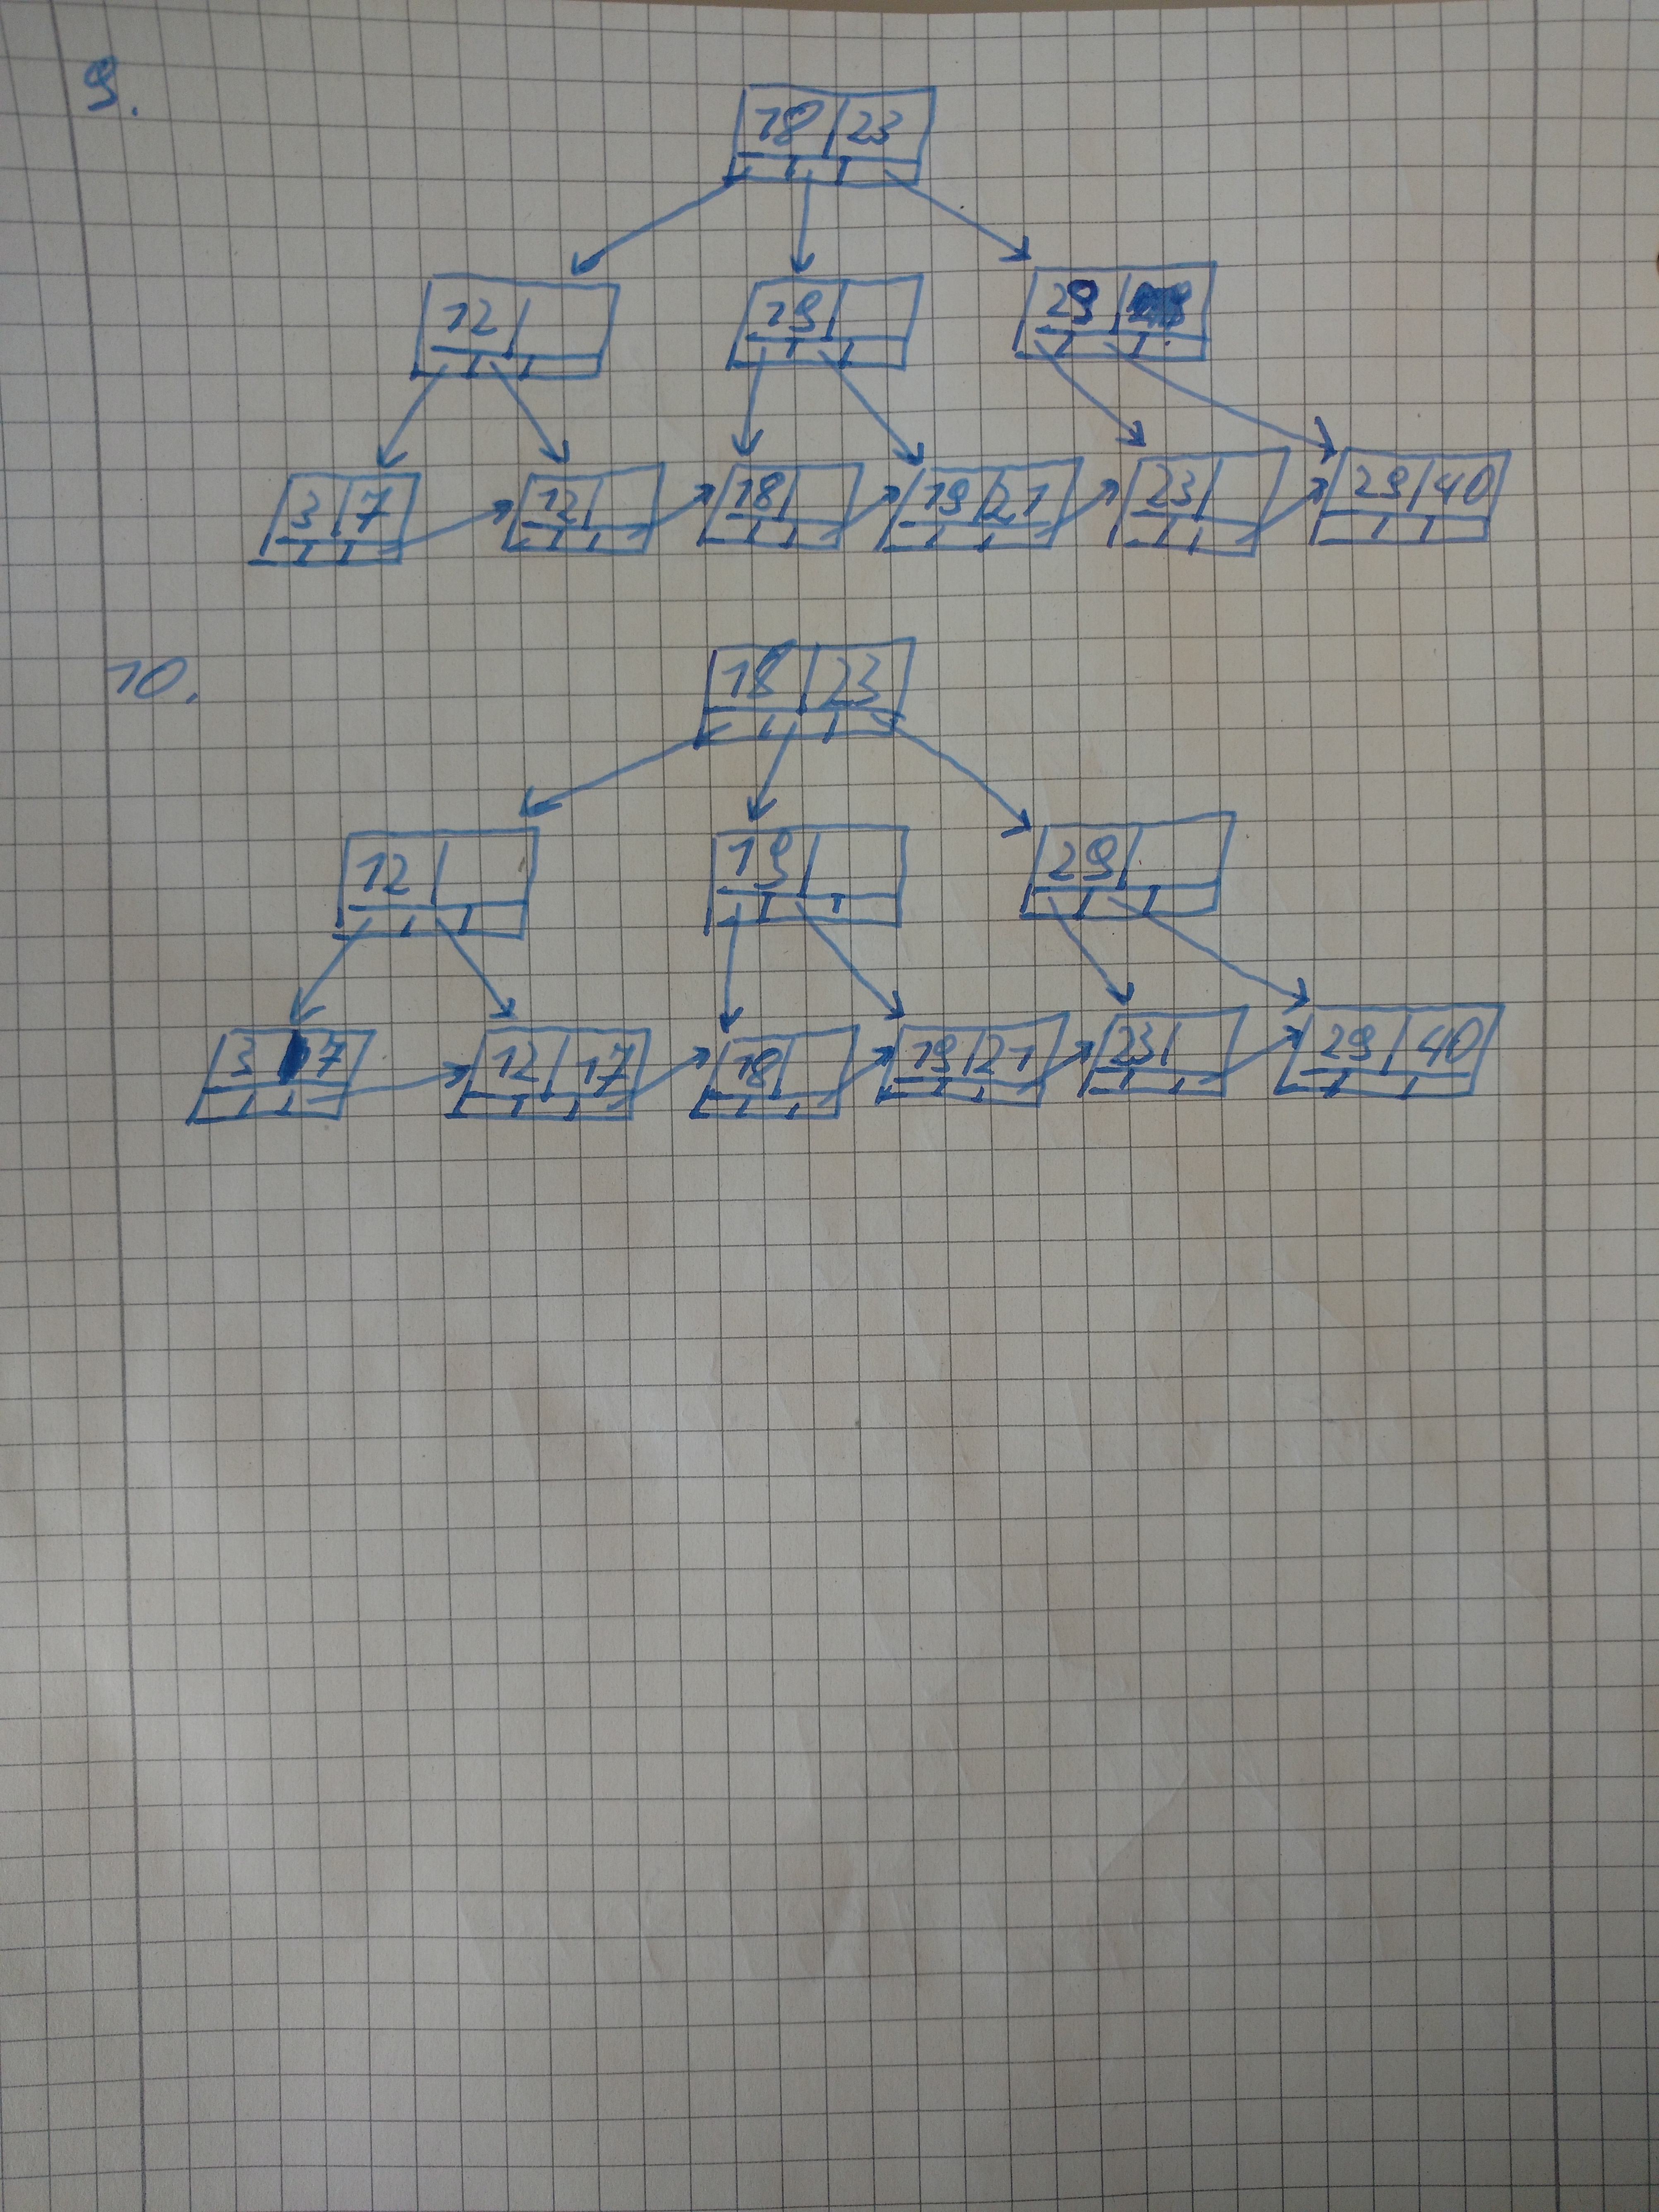
\includegraphics[width=\textwidth]{./images/a2.jpg}

\item[b)]

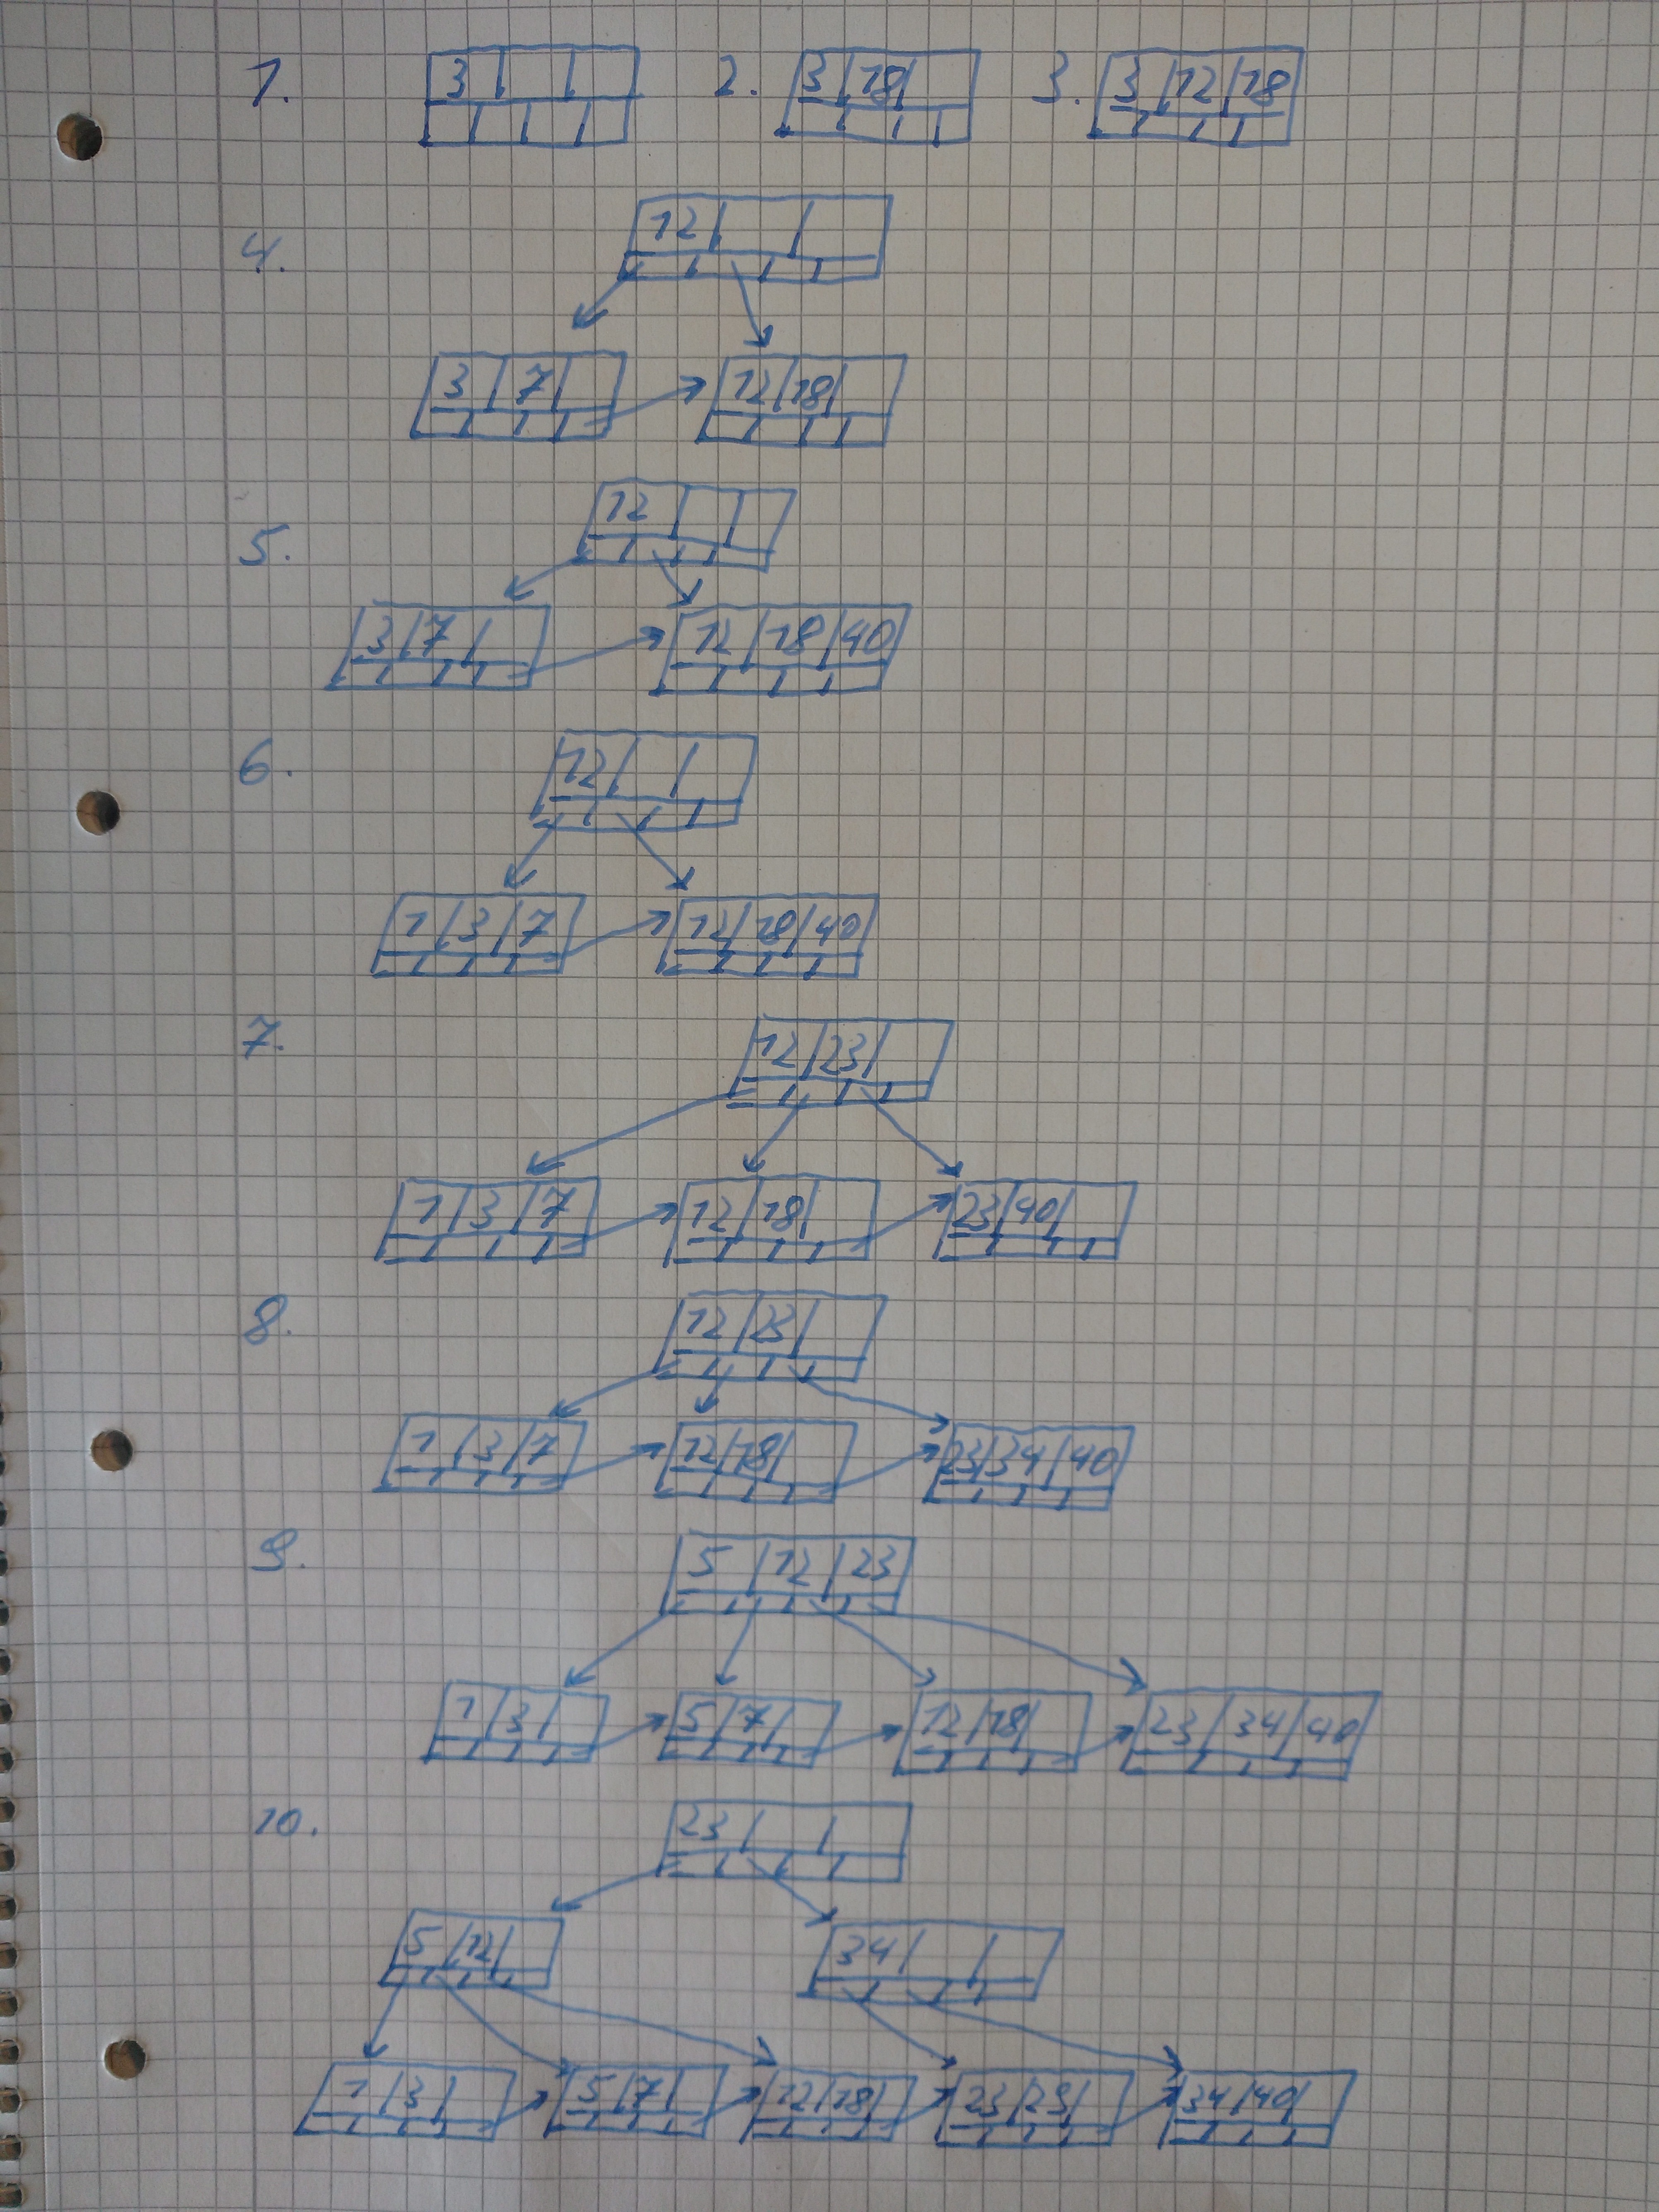
\includegraphics[width=\textwidth]{./images/b1.jpg}

\item[c)]

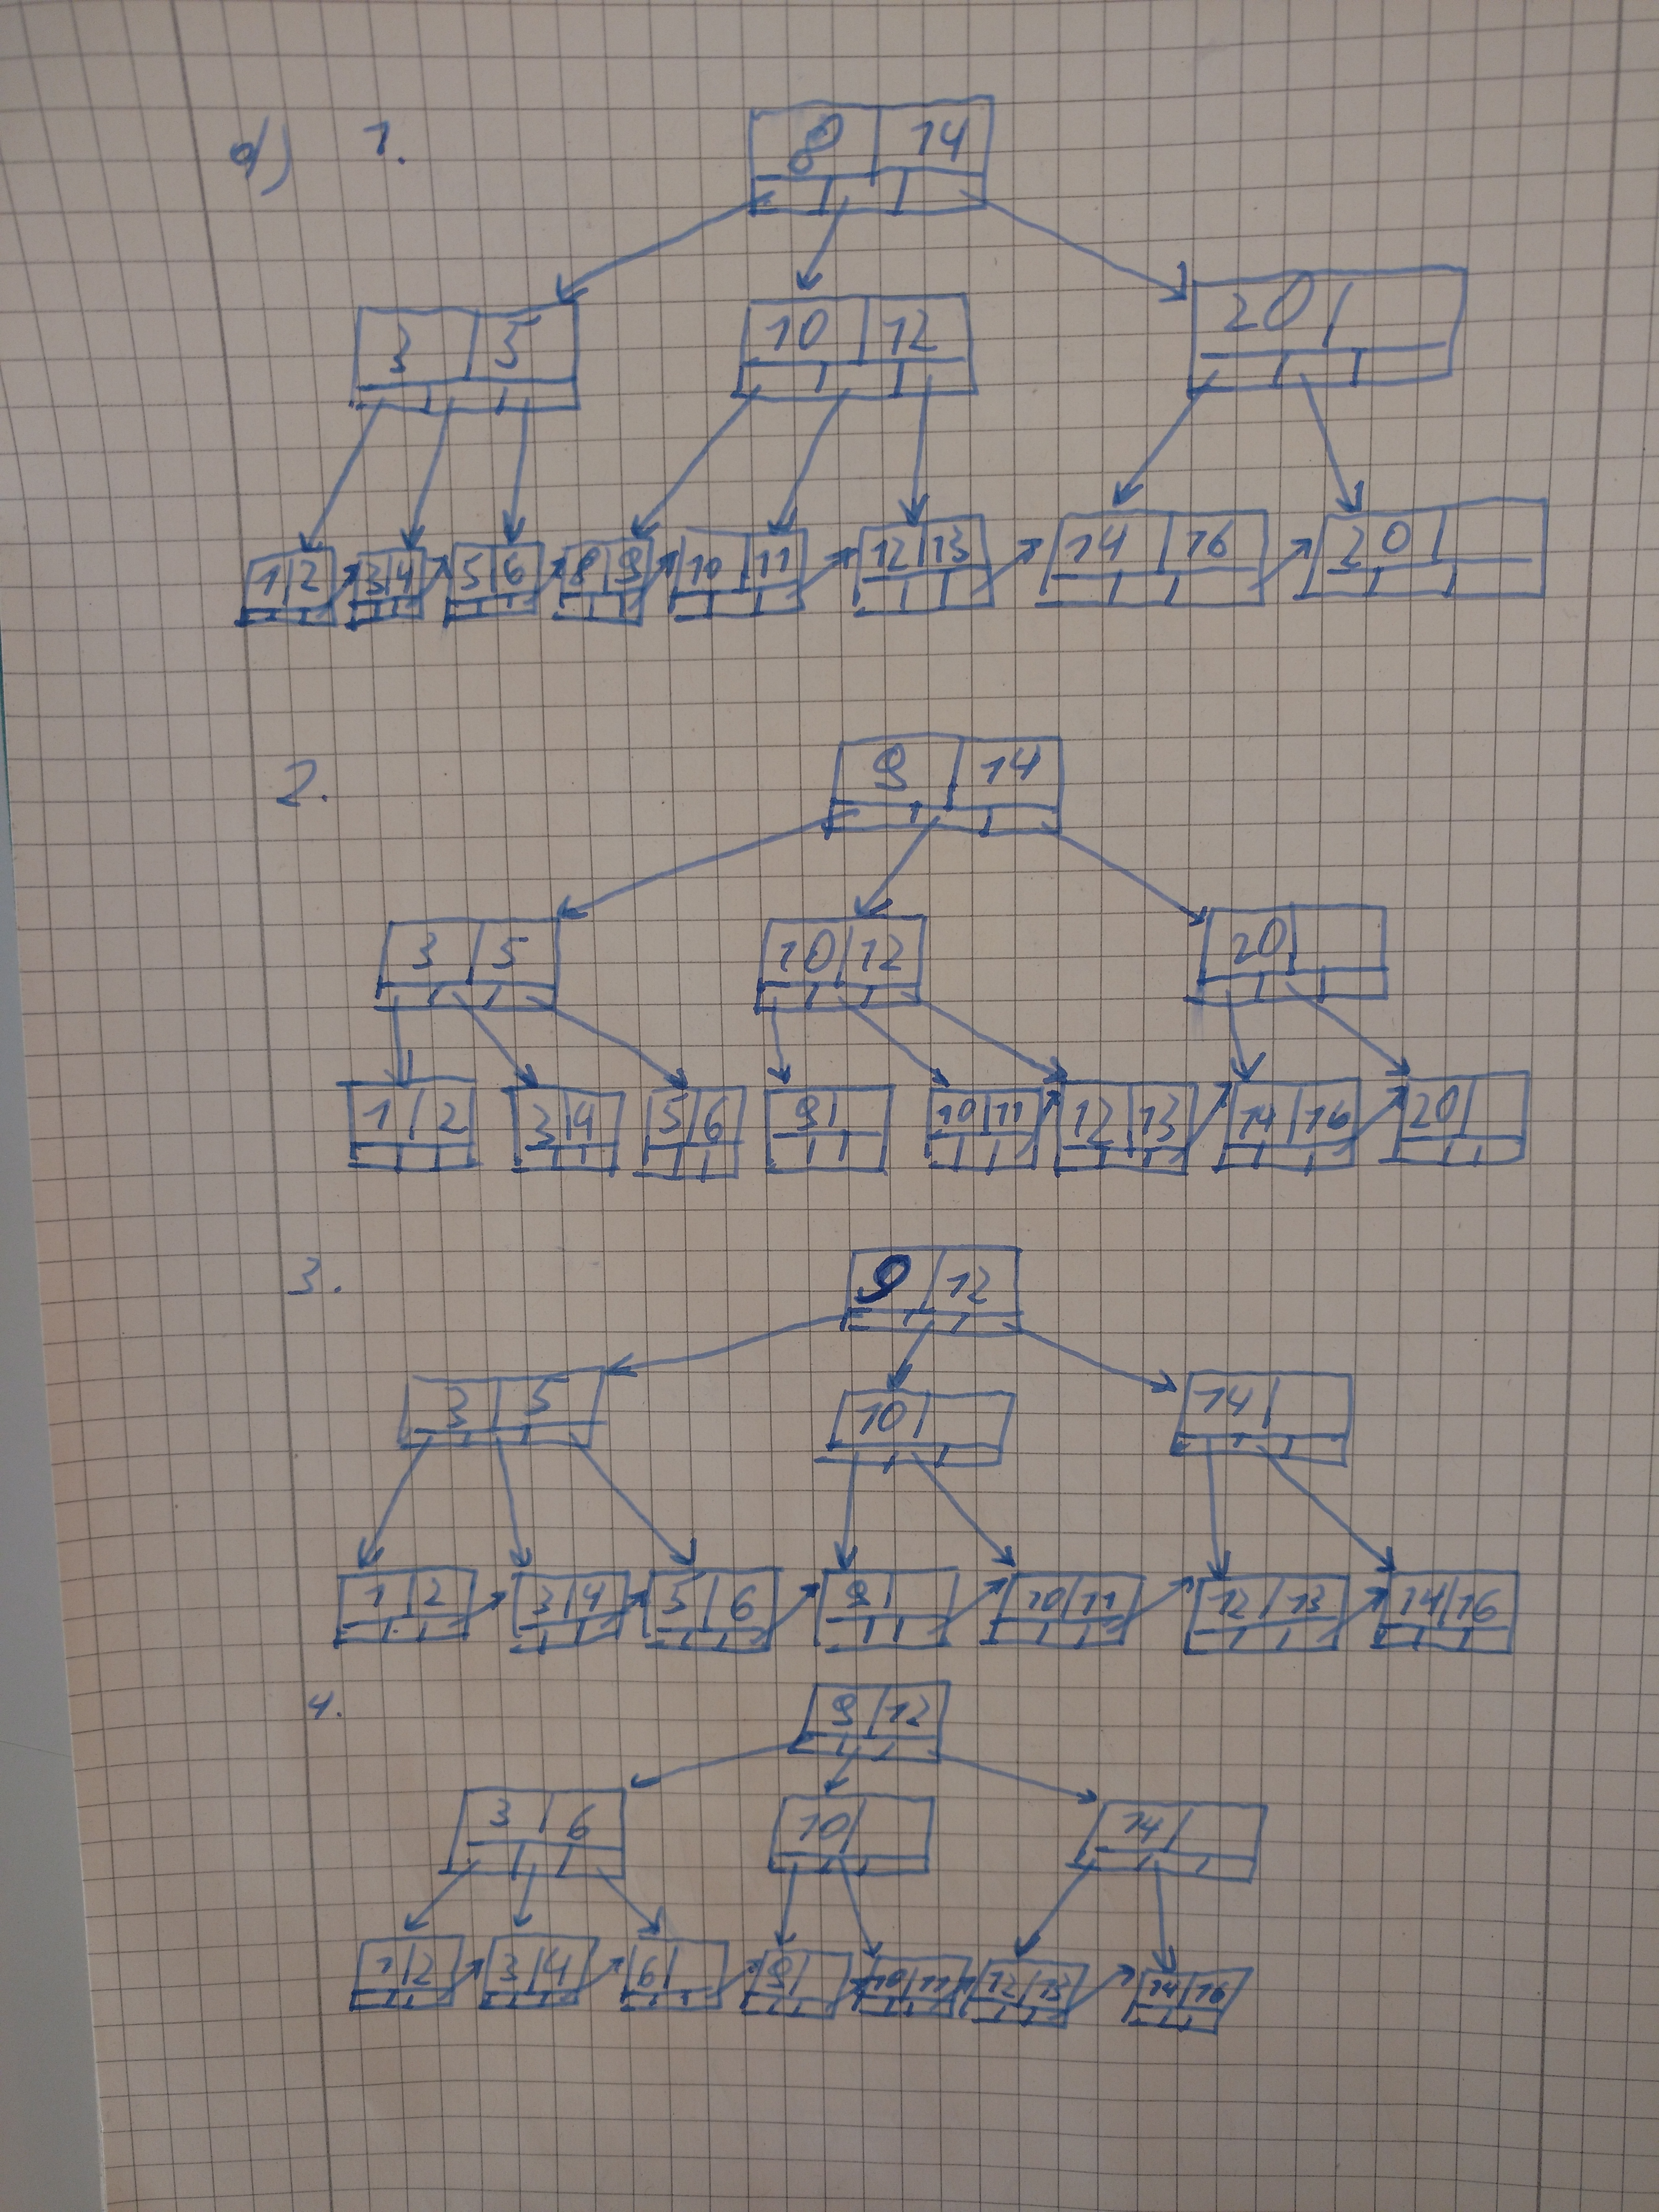
\includegraphics[width=\textwidth]{./images/c1.jpg}
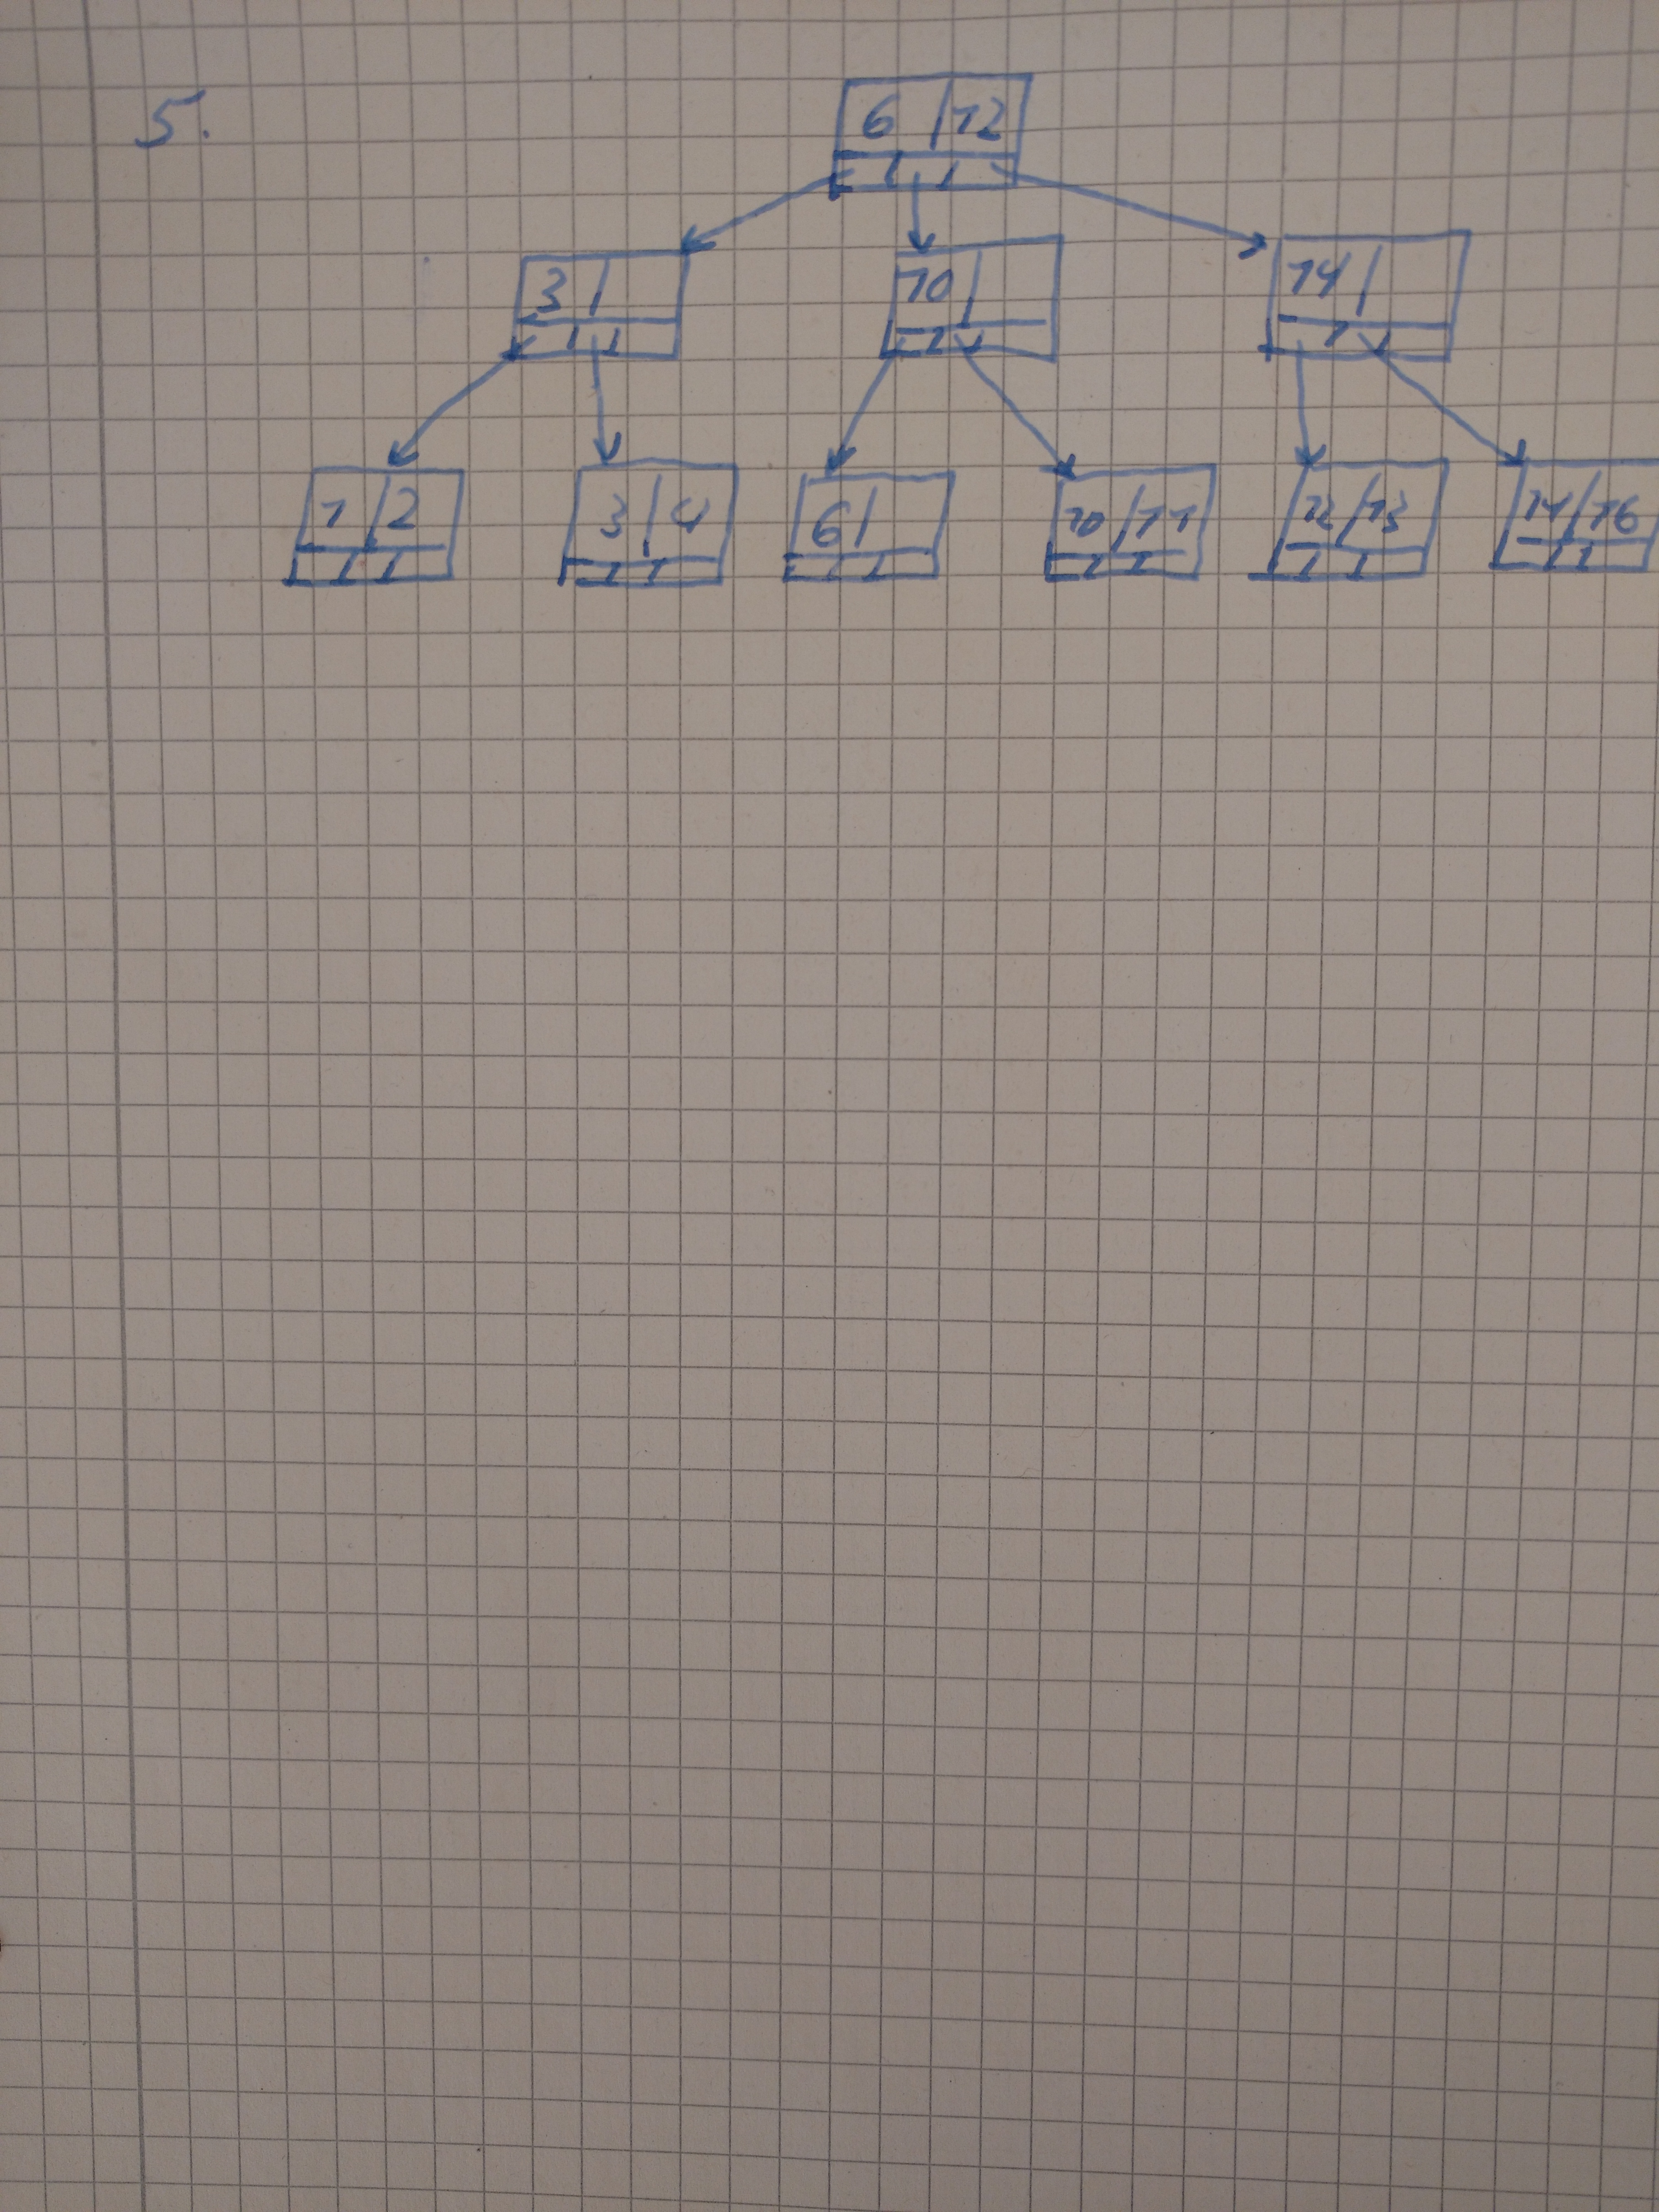
\includegraphics[width=\textwidth]{./images/c2.jpg}

\end{enumerate}

% /////////////////////// END DOKUMENT /////////////////////////
\end{document}
